One of the challenges of multi-agent systems is making sure that the agent will not behave in an unacceptable or undesirable way.
Agents may act in complex production environments, where failure of a single agent may cause serious losses.
Formal methods have been used in computer science as a basis to solve correctness challenges.
They represent agents as a high-level abstractions in complex systems.
Such a representation can lead to simpler techniques for design and development.

There are two roles of formal methods in distributed artificial intelligence that are often referred to.
Firstly, with respect to precise specifications they help in debugging specifications and in validation of system implementations.
Abstracting from specific implementation leads to better understanding of the design of the system being developed.
Secondly, in the long run formal methods help in developing a clearer understanding of problems and their solutions. \cite{Singh_99}

To formalise the concepts of multi-agent systems different types of logics are used, such as propositional, modal, temporal and dynamic logics.
In the following several paragraphs these logics, their properties and introduced operators will be briefly discussed.
Describing the details of interpretations and models of each individual logic is not the purpose of this report and is left out for further reading.

Propositional logic is the simplest logic and serves as the basis for logics discussed further in this section.
It is used to represent factual information and in our case is most suitable to model the agents' environment.
Formulas in this logic language consist of atomic propositions (represinting known facts about the world) and truth-functional connectives: $\land,\lor,\neg,\rightarrow$ which denote \enquote{and}, \enquote{or}, \enquote{not} and \enquote{implies}, respectively~\cite{Enderton_72}.

Modal logic extends propositional logic by introducing two different modes of truth: possibility and necessity.
In the study of agents, it is used to give meaning to concepts such as belief and knowledge.
Syntactically, modal operators in modal logic languages are defined as $\Diamond$  for possibility and $\Box$ for necessity.
The semantics of modal logics are traditionally given in terms of sets of so-called \emph{possible worlds}.
A world here can be interpreted as a possible state of affairs or sequence of states of affairs (history).
Different worlds can be related via a binary accessibility relations, which tells us which worlds are within the realm of possibility from the point of view of a given world.
In the sense of the accessibility relation, a condition is assumed \emph{possible} if it is true somewhere in the realm of possibility and it is assumed \emph{necessary} if it is true everywhere in the realm of possibility~ \cite{Saul_63}.

Dynamic logic is also referred to as modal logic of action.
It adds different atomic actions to the logic language.
In our case, atomic actions may be represented as actions that agents can perform directly.
This makes dynamic logic very flexible and useful for distributed artificial intelligence systems.
Necessity and possibility operators of dynamic logic are based upon the kinds of actions available~\cite{Kozen_90}.

Temporal logic is the logic of time.
There are several variations of this logic, such as:
\begin{description}
  \item[Linear] (or \emph{branching}): single course of history or multiple courses of history.
  \item[Discrete] (or \emph{dense}): discrete steps (like natural numbers) or always having intermediate steps (like real numbers).
  \item[Moment-based] (or \emph{period-based}): atoms of time are points or intervals.
\end{description}
We will concentrate on discrete moment-based models with linear past, but consider both linear and branching futures.

Linear temporal logic introduces several important operators. $p\cup q$ is true at a moment $t$ on a path, if and only if $q$ holds at a future moment on the given path and $p$ holds on all moments between $t$ and the selected occurrence of $q$.
$Fp$ means that $p$ holds sometimes in the future on the given path.
$Gp$ means that $p$ always holds in the future on the given path.
$Xp$ means that $p$ holds in the next moment.
$Pq$ means that $q$ held in a past moment~\cite{Singh_99}.

\begin{figure}[h!]
  \caption{An example branching structure of time~\cite{Singh_99}.}
  \centering
  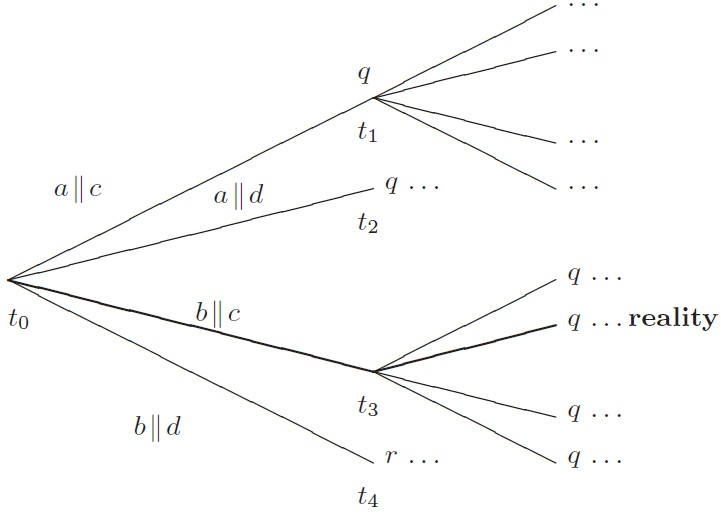
\includegraphics[width=0.6\textwidth]{images/branching_logic.png}
  \label{fig:for_branching_figure}
\end{figure}

Branching temporal and action logic is built on top of both dynamic and linear temporal logics and captures the essential properties of actions and time that are of value in specifying agents.
It also adds several specific branching-time operators.
$A$ denotes \enquote{in all paths at the present moment}.
The present moment here is the moment at which a given formula is evaluated.
$E$ denotes \enquote{in some path at the present moment}.
The reality operator $R$ denotes \enquote{in the real path at the present moment}.
\autoref{fig:for_branching_figure} illustrates the example of branching time for two interacting agents.

For modeling intelligent agents, quite often the BDI concept is used, which was described earlier in this report.
BDI stands for three cognitive specifications of agents: beliefs, desires and intentions.
To model logic of these specifications we will need to introduce several modal operators: $Bel$ for beliefs, $Des$ for desires, $Int$ for intentions and $K_h$ for know-how.
Considering these operators, for example, the mental state of an agent who desires to win the lottery and intends to buy a lottery ticket sometime, but does not believe that he will ever win can be represented by the following formula: $DesAFwin \land IntEFbuy \land \neg BelAFwin$.
For simplification in future we will consider only those desires which are mutually consistent.
Such desires are usually called goals.

It is important to note several important properties of intentions, which should be maintained by all agents~\cite{Singh_92}:
\begin{description}
  \item[Satisfiability] $xIntp\rightarrow EFp$.
    This means that if $p$ is intended by $x$, then it occurs eventually on some path.
    An intention following this condition is assumed to be satisfiable.
  \item[Temporal consistency] $(xIntp \land xIntq)\rightarrow xInt(Fp \land Fq)$.
    This requires that if an agent intends $p$ and intends $q$, then it (implicitly) intends achieving them in some undetermined temporal order: $p$ before $q$, $q$ before $p$, or both simultaneously.
  \item[Persistence does not entail success] $EG((xIntp) \land \neg p)$ is satisfiable.
    This is quite intuitive: just because an agent persists with an intention does not mean that it will succeed.
  \item[Persist while succeeding] This constraint requires that agents desist from revising their intentions as long as they are able to proceed properly.
\end{description}

The concepts introduced above may be used in each of the two roles of formal methods introduced earlier.
The two most commonly used reasoning techniques to decide an agent's actions are theorem proving and model checking.
The first one is more complex in terms of calculations, when the second one is more practical, but it requires additional inputs, though it does not prove to be a problem in several cases.

Considering the practical implementation, the architecture of an abstract BDI-interpreter can be described as follows.
The inputs to the system are called events, and are received via an event queue.
Events can be external or internal in relation to the system.
Based on its current state and input events, the system selects and executes options, corresponding to some plans.
The interpreter continually performs the following: determine available options, deliberate to commit to some options, update the state and execute chosen atomic actions.
After that, it updates the event queue and eliminates the options which have already achieved or are no longer possible.

\todo{Add or leave out a caption for all listings. Currently we are not consistent with that.}
\begin{lstlisting}
  BDI-Interpreter
  initialise_state();
  do
    options := option-generator(event-queue, B, G, I);
    selected-options := deliberate(options, B, G, I);
    update-intentions(selected-options, I);
    execute(I);
    get-new-external-events();
    drop-successful-attitudes(B, G, I);
    drop-impossible-attitudes(B, G, I);
  until quit.
\end{lstlisting}

As was mentioned above, options are usually represented by plans.
Plans consist of of the name or type, the body usually specified by a plan graph, invocation condition (triggering event), precondition specifying when it may be selected and add list with delete list, specifying which atomic propositions to be believed after successful plan execution.
Intentions in this case may be represented as hierarchically related plans.

Getting back to the algorithm and assuming plans as options, the option generator may look like the following.
Given a set of trigger events from the event queue, the option generator iterates through the plan library and returns those plans whose invocation condition matches the trigger event and whose preconditions are believed by the agent.

\begin{lstlisting}[mathescape]
  option-generator(trigger-events, B, G ,I)
  options := {};
  for trigger-event $\in$ trigger-events do
    for plan $\in$ plan-library do
      if matches(invocation(plan, trigger-event) then
        if provable(precondition(plan), B) then
          options := options $\cup$ plan;
  return options.
\end{lstlisting}

Deliberation of options should conform with the execution time constraints, therefore under certain circumstances random choice might be appropriate.
Sometimes lengthy deliberation becomes possible by introducing meta-level plans into the plan library, which form intentions towards some particular plans.

\begin{lstlisting}[mathescape]
  deliberate(options)
  if length(options) $\leq$ 1 then return options;
  else metalevel-options :=
            option-generator(b-add(option-set(options)));
    selected-options := deliberate(metalevel-options);
    if null(selected-options) then
        return random-choice(options);
    else return selected-options.
\end{lstlisting}

Coordination is one of the core functionalities needed by multi-agent systems.
Especially when different agents act autonomously and have different roles and possible actions.

One of the approaches developed by Singh~\cite{Singh_97} represents each agent as a small skeleton, which includes only the events or transitions made by the agent that are significant for coordination.
The core of the architecture is the idea that agents should have limited knowledge about the designs of other agents.
This limited knowledge is called the significant events of the agent.
There are four main types of events:
\begin{itemize}
  \item flexible, which can be delayed or omitted,
  \item inevitable, which can only be delayed,
  \item immediate, which the agent is willing to perform immediately,
  \item triggerable, which the agent performs based on external events.
\end{itemize}
These events are organised into skeletons that characterise the coordination behavior of agents.
The coordination service is independent of the exact skeletons or events used by agents in a multi-agent system.

To specify coordinations, a variant of the linear-time temporal language with some restrictions is used.
Two temporal operators are introduced for this purpose: $\cdot$, which is the before operator, and $\bigodot$, which is the operator of concatenation of two time traces, the first of which is finite.
Such special logic allows a variety of different relationships to be captured.

Overall, formal methods provide a logic abstraction for multi-agent systems.
They help to find self-consistent models of an agent's behavior.
However, relatively high complexity does not allow these methods to be implemented in real-time systems.
Therefore, the role of formal methods nowadays is limited to debugging, validation and design purposes.

In our project we unfortunately did not apply any formal methods for debugging or validating, mostly because of the limited time for development.
